\section{CTA-Pipelining Protocol: Design, Integration with CUTLASS, and Overhead Analysis}

In this section, we present the design and implementation of the CTA-pipelining protocol. We demonstrate its integration into the state-of-the-art NVIDIA CUTLASS library for GEMM operations and provide a detail execution trace analysis to understand and quantify the protocol's overhead.

As a software approach built upon current hardware and CUDA programming capabilities, our inter-kernel communication relies on atomic counters and queues, sharing structural similarities with latest literatures~\cite{cusync2024,davies2025kitsune}. However, we distinguish our work by elevating this mechanism into a cross-device spatial scaling method, and provides the placement strategy and additional coherency-ensuring design for multi-GPU setup. Moreover, we present novel implementation of integrating the protocol into multi-stage warp-specialized persistent kernels, and provide novel finding that such integration can effectively hide protocol overhead. 

% Basic protocol
\subsection{Basic Protocol}

%% Picture: illustrate all the components and how they are placed across GPUs

% \begin{figure}
%     \includegraphics[width=\columnwidth]{fig/Overview.png}
%     \caption{The overview of execution in CTA-pipelining manner.}
%     \label{fig:cta-overview}

%     \Description{Something required by ACM}
% \end{figure}

As its name suggests, CTA-pipelining is designed to execute dependent GPU kernels in a deeply pipelined manner at the finest architectural granularity: the CTA. In this model, each CTA consumes one or more input data tiles and produces a single output tile. Rather than enforcing strict kernel-level synchronization, our approach allows the consumer kernel to launch its CTAs as soon as the producer kernel generates the requisite data tiles. The kernel execution trace is similar to Figure~\ref{fig:chunk-cta}, where data dependent kernels are spatially distributed across GPU compute resources, getting launched simultaneously, and complete almost at the same time, except the tail at the consumer kernel for the last wave of pipelined CTA computation. 

In single-GPU context, this goal is conceptually similar to the Megakernel~\cite{wu2024mirage,cheng2025mpk} approach, which recompiles the entire workload to execute a tile-level dependency graph on a single device. However, CTA-pipelining aims to enable fine-grained pipelined execution spatially across multiple GPUs while preserving the original kernel structure, without the need to recompile the overall workflow. To enable data-dependent kernels to launch concurrently across multiple GPUs while maintaining execution correctness, additional control-flow dependency organization is required.

\begin{figure}[t]
    \centering
    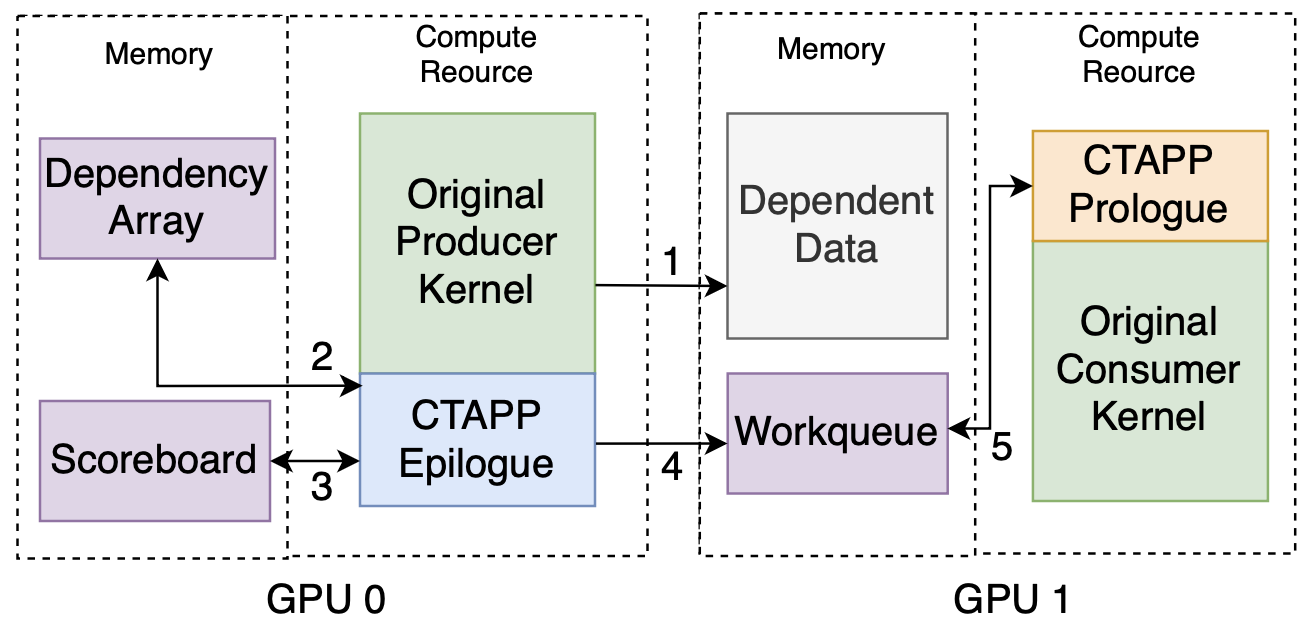
\includegraphics[width=\columnwidth]{fig/ctapp-setup.png}
    \caption{Setups of enabling CTA-pipelining across 2 GPUs.}
    \label{fig:ctapp-setup}
    \vspace{-3mm}

\end{figure}

Figure~\ref{fig:ctapp-setup} illustrates the overall execution process of CTA-pipelining, using a two-GPU setup to demonstrate how the original kernel interacts with the additional components. The underlying data structures that support this paradigm include dependency arrays, scoreboards, and inter-device workqueues, which we collectively refer to as \textit{dependency structure}. To interface with the dependency structure and orchestrate the control flow, lightweight prologues and epilogues are injected directly into the original kernel code. We detail each of these core components below, followed by a step-by-step execution walkthrough.


\subsubsection{Dependency Array}
The dependency array indicates the control-flow dependencies between producer CTAs and consumer CTAs. Specifically, it is indexed by the producer CTA ID to identify which consumer CTAs if affects, including a contiguous list of consumer CTA IDs and a corresponding offset array that defines the index range for each producer. These dependencies can be derived directly from data dependencies, using static analysis, trial runs of the kernels, or even calculated dynamically at runtime if closed-form formula exist. As the dependency array is exclusively accessed by consumer CTAs, it is stored on the producer device memory.

\subsubsection{Scoreboard}
To resolve many-to-one data dependencies, where a consumer CTA relies on output from multiple producer CTAs, a scoreboard is used to track producer completion. The scoreboard consists of an array of atomic counters, with each consumer CTA assigned an entry,  initialized to the total number of its prerequisite producer CTAs. A counter reaching zero serves as a readiness signal, indicating a consumer CTA is ready for execution. The scoreboard is initialized as part of the prior dependency analysis. Since the scoreboard is also exclusively modified by producer CTAs, it is stored on the producer device memory.

\subsubsection{Inter-device Workqueue}
The inter-device workqueue serves as a readiness signaling mechanism between the producer kernel and the consumer kernel. Implemented as a cyclic ring buffer, it is managed by several atomic values including head, tail, and size to ensure coherency. 

Since the workqueue requires concurrent access from both kernels, cross-device NVLink is utilized. We place the workqueue in the consumer device's memory to minimize critical-path latency. While cross-device writes are theoretically expensive, CUDA's asynchronous write semantics allow the producer to issue "fire-and-forget" memory operations without stalling for completion (unless there is explicit flush barrier). Conversely, consumer CTAs must continuously poll the workqueue, and forcing these frequent read operations across NVLink would incur latency penalties. Therefore, placing the workqueue on the consumer device is a more reasonable design choice.

\subsubsection{Overall Workflow with Prologue and Epilogue Code Snippets}

The data structures described above facilitate the CTA-pipelining control flow. The logic that utilizes these data structures consists of minimal prologue and epilogue code snippets. These are added to the beginning and end of the kernel code, leaving the core original kernel implementation untouched. (Warp-specialized kernels are treated slightly differently, as introduced later.)

The overall control flow orchestrated by the injected prologue and epilogue is illustrated by the numbered arrows in Figure~\ref{fig:ctapp-setup}. First, the producer CTA writes its output directly to the consumer's input memory across NVLink, as indicated by arrow (1). Its epilogue then issues a system-wide memory fence, ensuring subsequent dependency operations and workqueue updates do not become visible to other devices before the actual output data is visible. After that, it utilizes SIMD execution to atomically decrement dependency counters in scoreboard after querying dependency array (2, 3). When a counter reaches zero, the producer thread pushes the ready consumer CTA ID into workqueue (4). On the consumer side, the injected prologue uses a single thread to busy-poll this workqueue while the remaining threads wait at a barrier (5). Upon retrieving a ready ID, the polling thread broadcasts it via shared memory. The consumer CTA then remaps its ID to this fetched value and executes its standard, unmodified kernel payload.


% The overall control flow enabled by add-on prologue and epilogue are illustrated by number and arrows in Figure~\ref{fig:ctapp-setup}. First, the producer kernel CTA executes as it originally does, writing output data directly to the input buffer of consumer kernel across NVLink, as indicated by 1 in the figure. Second, the add-on CTA-pipelining Epilogue code issue a system-wide threadfence to ensure that subsequent dependency operations and workqueue updates do not become visible to other devices before the actual output data is visible. After that, it queries the dependency to find out the consumer CTA that it affects, as indicated by 2. Third, Using these IDs as indices, it atomically decrements the remaining dependency counters in the scoreboard with SIMD execution. Forth, If a scoreboard counter reaches 0, the corresponding consumer CTA is ready to execute; the specific producer thread that decremented the counter to 0 is then responsible for pushing the ready CTA ID into the workqueue.

% The workflow then continues to the consumer side. With the prologue placed before the original consumer kernel code, each CTA uses a single thread to busy-poll the workqueue, interleaved with brief sleep intervals, while the remaining threads wait at a barrier, as indicated by arrow 5. Once the polling thread retrieves a ready CTA ID, it broadcasts it via shared memory. The subsequent CTA execution remains unmodified, except for a CTA ID remapping process: the CTA adopts the new ID fetched from the workqueue to guide all of its subsequent computations.

% {\tt \small
% \begin{verbatim}
% #include <iostream>
% using namespace std;
% main()
% {
% cout << "Hello world \n";
% return 0;
% }

% \end{verbatim}
% }


\subsubsection{Host-Side Organization}

From the host side, each kernel is assigned a dedicated CUDA stream and bound to a specific device or a partition of devices. During execution, all kernels are launched simultaneously, with internal execution order dynamically guided by the CTA-pipelining protocol. In multi-layer workloads, intermediate kernels act as both producers and consumers. These kernels feature both a prologue to fetch from an source workqueue and an epilogue to push to a destination workqueue. Note, this entire multi-kernel execution process can be captured by CUDA Graphs, reducing kernel launching bubbles. 

In actual workflows, the CUDA driver's default CTA scheduling order might not allow the entire workload to execute in a smoothly pipelined manner. In such cases, altering the execution order, such as shifting from a column-major to a row-major pattern, can be beneficial. In this case, the first kernel in the workflow can simply consume a pre-defined source workqueue to explicitly guide its CTA execution order.

There is an optional micro-optimization to eliminate the SM resource waste of initial busy-polling, using \textit{cuStreamWaitValue32} API. This feature blocks the consumer's execution stream until the workqueue contains at least one item, preventing immediate spin-waiting. However, this stream-level synchronization does incur a slight latency penalty for the kernel launch.

% TODO: automation

\subsection{Integration with CUTLASS GEMM Kernels}

In this subsection, we explain how the CTA-pipelining protocol can be integrated into two different styles of GPU kernels, using NVIDIA CUTLASS GEMM implementations~\cite{cutlass} as examples. To illustrate the dependency mapping, we use a two-layer GEMM workload as our running example, where the output of the first GEMM is directly consumed by the subsequent GEMM. 

\subsubsection{Classical Kernels}

As a straightforward example, we demonstrate how CTA-pipelining integrates with classical GEMM kernels, using the SM90 TMA kernel from the CUTLASS library. In this kernel, each CTA has all threads follow the same execution flow, producing one tile of the output matrix. At the end of its execution, the CTA terminates, and the next wave of CTAs is scheduled by the CUDA driver. This represents the most classical GPU kernel structure.

% \begin{figure}
%     \caption{GEMM to GEMM dependency}
% \end{figure}
% The dependency analysis for a two-layer GEMM workload is shown in Figure~\ref{}, providing a specific example with defined matrix and tile sizes. 

In terms of control dependencies, each consumer CTA computes one output tile by consuming an entire row of input tiles, making it dependent on an entire row of producer CTAs. Furthermore, consumer CTAs in the same row share identical dependencies. While we recognize that this could be simplified to a row-to-row dependency rather than a strict CTA-to-CTA dependency, or calculated dynamically at runtime using matrix and tile dimensions, we present the most general case for illustrative purposes.

Regarding modifications to the CUTLASS library, integrating CTA-pipelining protocol is minimally invasive. Beyond extending the parameter structure to accept the necessary dependency structures, the source code changes are restricted to injecting the prologue and epilogue snippets. Notably, while the prologue requires shared memory to broadcast the dynamically fetched CTA ID to all threads, it reuses the memory space already allocated for the kernel's main execution. This does not affect the subsequent execution, as the prologue runs at the very beginning of the kernel and its shared memory usage is strictly one-time.

In summary, integrating CTA-pipelining with classical kernels is highly straightforward. It does not require a detailed understanding or modification of the core execution logic, demonstrating that this approach is highly generalizable to other kernels.

\subsubsection{Warp-Specialized Multi-Stage Persistent Kernels}

The warp-specialized multi-stage persistent kernel is a representative example of programming models evolution and serves as the foundational design for modern high-performance libraries like CUTLASS. As its structural paradigm differs from classical kernels, it is helpful to demonstrate how CTA-pipelining integrates with this kernel design, using SM100 TMA Warp Specialized kernel from CUTLASS as an example. 

This architecture relies on three important concepts. First, \textit{persistent kernels} launch a fixed number of CTAs that remain active for the entire computation, dynamically fetching work-tiles via explicit metadata rather than relying on standard CTA IDs. Second, a \textit{multi-stage} design divides the workflow into an internal micro-pipeline. Third, \textit{warp specialization} assigns these distinct micro-pipeline stages to independent warps of threads.


% To provide necessary background, we provide a brief introduction to three important concepts involved: persistent, multi-stage, and warp-specialized. First, a persistent kernel launches a fixed number of CTAs, typically matching the maximum hardware occupancy, which remain active for the duration of the entire computation. Instead of terminating upon completing a task, these CTAs dynamically fetch the next work item until all work is exhausted. Consequently, workload mapping relies on explicit work-tile metadata rather than standard hardware-assigned CTA IDs. Second, a multi-stage design explicitly divides the computational workflow into distinct phases, forming an internal micro-pipeline. Third, warp specialization is one execution model for multi-stage kernels, assigning these distinct micro-pipeline stages to independent warps, as different warps are executed independently by the hardware.

In the SM100 CUTLASS implementation, these three concepts operate together. The resulting micro-pipeline includes discrete stages for scheduling, main data loading, Matrix Multiply-Accumulate (MMA), GEMM epilogue data loading, and GEMM epilogue operations. One dedicated warp handles each stage, except the GEMM epilogue stage might have multiple warps.  

The CTA-pipelining prologue is integrated directly into the scheduler warp. In the original SM100 CUTLASS kernel, information regarding the next work tile is obtained via a hardware query, known as a Cluster Launch Control (CLC) query, issued by a single thread within the scheduler warp to fetch the next ready work ID. Subsequently, the returned information is multicast across the CGA and stored in each CTA's Distributed Shared Memory (DSMEM). After this broadcast, each active warp decodes the response to extract the index of its next work tile.

Aligning with this native kernel structure, the CTA-pipelining prologue reuse this work-tile fetching and broadcasting pathway. Instead of issuing a hardware CLC query, the scheduling thread performs busy-polling on the added workqueue. Once it successfully fetches a work item from the queue, it issues remote memory stores to the DSMEM across the CGA, reusing the buffer originally allocated for the CLC response. Since the scheduler tracks the total number of tiles to be executed, it uses this information to determine the completion of the workload by comparing the current workqueue index against the total tile count. The other compute warps fetch the next work tile similar to before, but changing the decoding format for the new metadata structure.

The CTA-pipelining epilogue is positioned at the final stage of the micro-pipeline: the GEMM epilogue. In the SM100 CUTLASS GEMM implementation, multiple warps are used to execute arithmetic operations, while only one warp performs the final output write to global memory. As the global threadfence that ensures consistent memory views is only effective for each calling thread, only the specific warp responsible for writing global output issues the threadfence, and only this warp is utilized for the CTA-pipelining epilogue operations. The specific operations performed on the dependency structure remain identical to before.

A special case arises with Blackwell's specific Tensor Core operations, where two CTAs cooperatively issue a single Tensor Core instruction. In the CUTLASS GEMM implementation, this is reflected as a change in the tile ID mapping: while each CTA still receives separate work-tile information, the total tile size is doubled along one dimension to accommodate the CTA-pair operation. To handle this special case, the work-tile information fetched from the workqueue are decoded differently, and the scoreboard tracking values are adjusted accordingly. All other parts of the pipelining logic remain unchanged.

\subsection{Protocol Overhead on CUTLASS}

The first question that naturally arises is how the additional operations introduced by the CTA-pipelining protocol affect overall performance. To understand this impact, we investigate detailed execution phases and profile the latency of each operation by injecting timestamping code into the kernel, and perform analysis based on the collected timestamps. We present results for both classical kernels and warp-specialized multi-stage persistent kernels, as they exhibit different performance patterns. 

The evaluation of the classical SM90 CUTLASS kernel is performed on a 8-GPU H200 system, with GPUs connected by the $4^{th}$ generation NVLink. The SM100 TMA Warp Specialized kernel is evaluated on a 8-GPU B200 system, where GPUs are connected by the $5^{th}$ generation NVLink. For all evaluation on protocol overhead, all GEMM input sizes are 16384 by 8192, multiplying with weight matrix of 8192 by 8192. The input and output data types are set to BF16, and the Tensor Core accumulator type is set to FP32. The specific CUTLASS configuration is selected by running the CUTLASS Profiler~\cite{cutlass} on the given input size, and selecting the configuration with the fastest execution time.  

\begin{figure}[b]
    \centering
    
    \begin{subfigure}[b]{0.9\columnwidth}
        \centering
        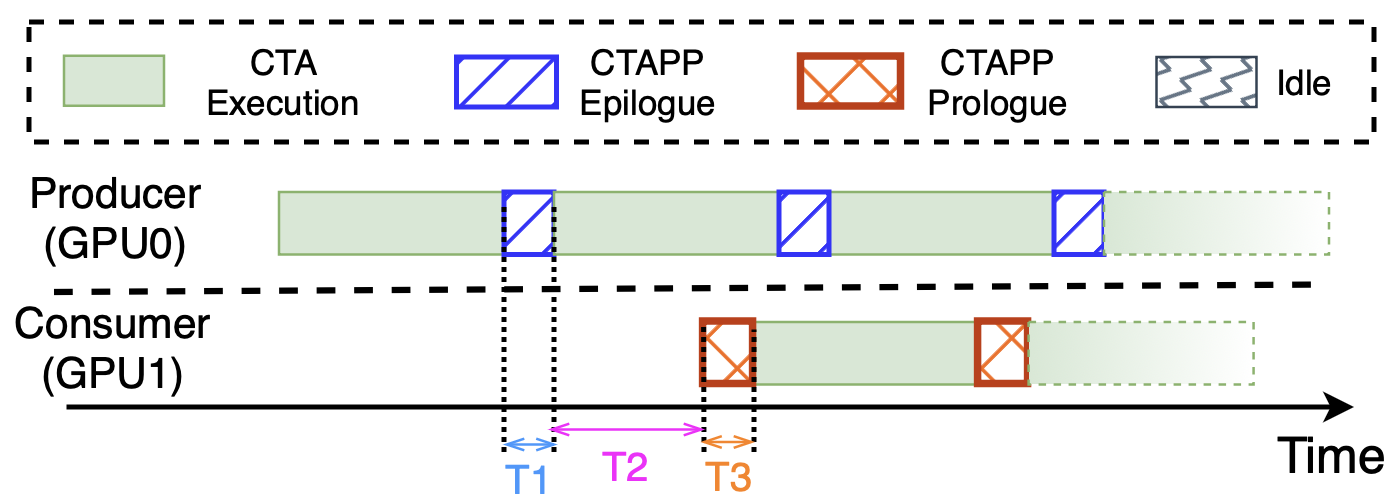
\includegraphics[width=\columnwidth]{fig/pic-basic.png}
        \caption{}
        \label{fig:pic-basic}
    \end{subfigure}

    \begin{subfigure}[b]{0.9\columnwidth}
        \centering
        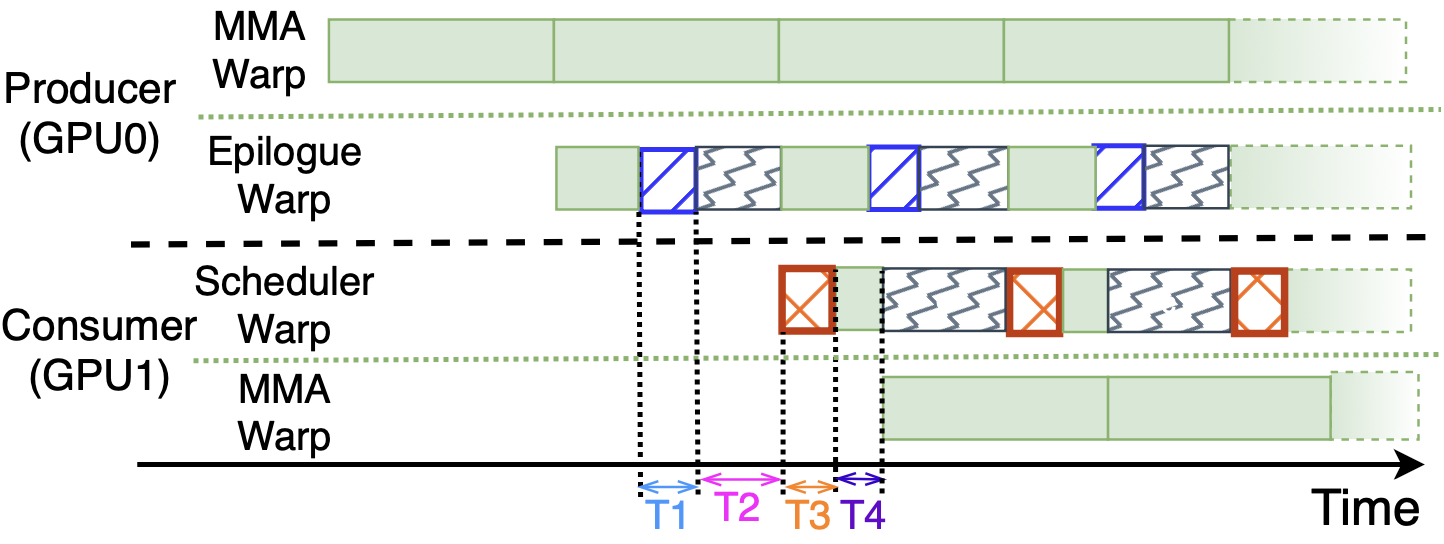
\includegraphics[width=\columnwidth]{fig/pic-warp.png}
        \caption{}
        \label{fig:pic-warp}
    \end{subfigure}
    
    \caption{The detail execution trace of adding CTA-pipelining to (a) classical kernel, and (b) warp-specialized multi-stage persistent kernel. For illustration purpose, time is not at the correct scale.}
    \label{fig:pic}

    \vspace{-3mm}

\end{figure}

For the classical kernel, the profile of the execution phases is shown in Figure~\ref{fig:pic-basic}. For each CTA, the epilogue operations take about T1=6$\mu$s. Subsequently, it takes T2=120$\mu$s for this update to become visible to the consumer device. On the consumer side, the prologue takes about T3=1.5$\mu$s to fetch the work queue value and broadcast the fetched information. Notice, this overhead accumulates for each wave of CTA execution.

The warp-specialized persistent kernel exhibits dramatically different results. CTA-pipelining can utilize the idle time of specific warps, effectively hiding its protocol overhead. As introduced earlier, the warp-specialized kernel inherently functions as a micro-pipeline. Since the entire pipeline is typically dominated by the latency of the compute-heavy MMA operations, the other warps frequently need to wait at pipeline barriers. This presents an opportunity to perform additional work within these waiting warps, such as the CTA-pipelining operations, without affecting overall performance. 

The exact execution trace for the warp-specialized persistent kernel is illustrated in Figure~\ref{fig:pic-warp}, including only the related warps for analysis. For each wave of execution, the epilogue operations, including the threadfence, take approximately T1=6$\mu$s. During this time, other warps remain active for the next wave of computation. By the time the next computational wave reaches the GEMM epilogue warp, the CTA-pipelining epilogue operations from the previous wave have already finished, allowing the warp to take on the next wave immediately, which hides the CTA-pipelining operation overhead. The cross-device NVLink data write takes roughly T2=5$\mu$s to become visible on the consumer device. On the consumer side, the prologue work queue fetching takes about T3=1.5$\mu$s, and it takes about T4=0.5$\mu$s to broadcast across the CGA by the scheduler warp. Similarly, since the scheduler warp is an stage of the micro-pipeline, this latency is also hidden. As a result, assuming no other memory or communication contention, the CTA-pipelining overhead is theoretically only visible once during the initial pipeline ramp-up.

As the CTA-pipelining logic is confined to the injected prologue and epilogue, it also imposes minimal performance interference on the original kernel. It does not disrupt the main compute phase's active register allocation or shared memory usage, avoiding register spilling or shared memory contention. For instance, in our evaluation of SM100 TMA Warp Specialized kernel, the baseline execution of two consecutive GEMMs takes an average of 1080$\mu$s each. When executed using CTA-pipelining, the producer completes in 1090$\mu$s, and the consumer finishes in 1165$\mu$s, counting in both the visible overhead and the latency of the final pipeline wave.

In summary, the overhead introduced by the CTA-pipelining protocol is minimal, and it can even be largely hidden within warp-specialized persistent kernels, making it suitable for general fine-grain spatial pipelining. We demonstrate more scaling examples with performance analysis in the next section. 
